% --------------------------------------------------------------------------------

\begin{exercise}

Zum asymptotischen Vergleich von Folgen:

\begin{enumerate}[label = (\alph*)]

  \item Vergleichen Sie das asymptotische Verhalten von $f(n) = n!$ und $g(n) = (n + 2)!$, also überlegen Sie sich ob eine (welche) der Funktionen ein $\landau, \Landau, \omega, \Omega, \Theta$ der anderen Funktion ist.

  \item Vergleichen Sie das asymptotische Verhalten von $f(n) = n^{\log_2(4)}$ und $g(n) = 3^{\log_2(n)}$, also überlegen Sie sich ob eine (welche) der Funktionen ein $\landau, \Landau, \omega, \Omega, \Theta$ der anderen Funktion ist.

  \item Zeigen Sie an Hand der Defintion, dass für positive Funktionen $f$ und $g$ die Beziehung

  \begin{align*}
    \max \Bbraces{f(n), g(n)} = \Theta(f(n) + g(n))
  \end{align*}

  gilt.

  \item Gilt selbige Beziehung ebenfalls für $\min \Bbraces{f(n), g(n)}$?

  \item Folgt aus $f(n) = \Landau(g(n))$, dass $2^{f(n)} = \Landau(2^{g(n)})$?

  \item Gilt für alle positiven Funktionen $f$ die Beziehung $f(n) = \Landau(f(n)^2)$?

  \item Finden Sie eine Funktion $f$, sodass weder $f(n) = \Landau(n)$ noch $f(n) = \Omega(n)$ gilt.

\end{enumerate}

\end{exercise}

% --------------------------------------------------------------------------------

\begin{solution}

\phantom{}

\begin{comment}

\includegraphicsboxed{Definition 1-4.png}
\includegraphicsboxed{Definition 1-5.png}
\includegraphicsboxed{Lemma 1-2.png}
\includegraphicsboxed{Lemma 1-3.png}

\end{comment}

\begin{enumerate}[label = (\alph*)]

  \item

  \begin{align*}
    \frac{f(n)}{g(n)} = \frac{n!}{(n+1)!} = \frac{1}{(n+2)(n+1)} \xrightarrow{n \to \infty} 0 \\
  \end{align*}

  \begin{align*}
    \stackrel{1.3.7}{\iff}
    f \in \landau(g)
    \stackrel{1.3.1}{\subseteq}
    \Landau(g) \\
    \stackrel{1.3.5}{\iff}
    g \in \omega(f)
    \stackrel{1.3.1}{\subseteq}
    \Omega(f)
  \end{align*}

  \begin{align*}
    \implies
    \frac{g(n)}{f(n)} \xrightarrow{n \to \infty} \infty
  \end{align*}

  \begin{align*}
    \stackrel{1.2.3}{\iff}
    g \not \in \Landau(f)
    \stackrel{1.3.2}{\supseteq}
    \landau(f) \\
    \stackrel{1.2.2}{\iff}
    f \not \in \Omega(g)
    \stackrel{1.3.2}{\supseteq}
    \omega(g)
  \end{align*}

  \begin{align*}
    \implies
    g
    \not \in
    \Landau(f) \cap \Omega(f)
    \stackrel{2.1.1}{=}
    \Theta(f) \\
    \implies
    f
    \not \in
    \Landau(g) \cap \Omega(g)
    \stackrel{2.1.1}{=}
    \Theta(g)
  \end{align*}

  \item

  \begin{align*}
    \log_2{4}               & = \log_2{2^2} = 2 \\
    \log_2{n}               & = \frac{\log_3{n}}{\log_3{2}} \\
    2 - \frac{1}{\log_3{2}} & > 0 \iff 2 > \frac{1}{\log_3{2}} \iff \log_3{4} = \log_3{2^2} = 2 \log_3{2} > 1 = \log_3{3^1}
  \end{align*}

  \begin{align*}
    \implies
    \frac{f(n)}{g(n)}
    =
    \frac{n^{\log_2{4}}}{3^{\log_2{n}}}
    =
    n^2 / \pbraces{3^{\log_3{n}}}^{1 / \log_3{2}}
    =
    n^{2 - \frac{1}{\log_3{2}}}
    \xrightarrow{n \to \infty} \infty
    \implies
    \frac{g(n)}{f(n)}
    \xrightarrow{n \to \infty} 0
  \end{align*}

  (b) ist also (a), verkehrt rum.

  \item

  \begin{comment}

    \begin{figure}[h!]
    \begin{boxedin}
      \vspace{0.5 cm}
      \hspace{0.5 cm}
      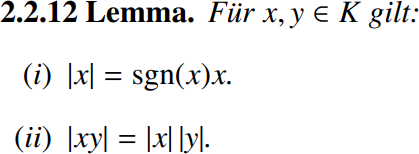
\includegraphics[width = 5 cm]{Kaltenbaeck - Fundament Analysis - Lemma 2-2-12-1.png} \\
      \vspace{0.01 cm}
      \hspace{0.5 cm}
      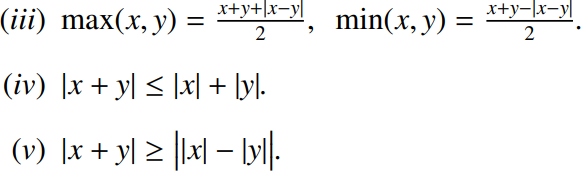
\includegraphics[width = 7 cm]{Kaltenbaeck - Fundament Analysis - Lemma 2-2-12-2.png} \\
      \vspace{0.5 cm}
      \caption{Kaltenbaeck - Fundament Analysis}
      \label{fig:KFAL2.2.12}
    \end{boxedin}
  \end{figure}

  \end{comment}

  Seien $c := 1/2$ und $d := 1$, dann gilt $\ForAlmostAll n \in \N:$

  \begin{multline*}
    c (f(n) + g(n))
    \leq
    \max \Bbraces{f(n), g(n)}
    =
    \frac{f(n) + g(n) + |f(n) - g(n)|}{2} \\
    \leq
    \frac{f(n) + g(n)}{2}
    +
    \frac{f(n) + g(n)}{2}
    =
    d (f(n) + g(n)).
  \end{multline*}

  \item Gegenbeispiel:
  Seien $f \equiv 0$ und $g \equiv 1$, dann gilt $\Forall c, d > 0:$

  \begin{align*}
    c \underbrace{(f(n) + g(n))}_1
    \not \leq
    \underbrace{\min \Bbraces{f(n), g(n)}}_0
    <
    d \underbrace{(f(n) + b(n))}_1.
  \end{align*}

  \begin{align*}
    \implies
    \min \Bbraces{f, g} \not \in \Theta(f + g)
  \end{align*}

  \item Gegenbeispiel:
  Seien $f(n) = n$ und $g(n) = -n$, für $n \in \N$, dann gilt wegen $|f| = |g|$ zwar $f \in \Landau(g)$, aber

  \begin{align*}
    \limsup_{n \to \infty}
    \vbraces
    {
      \frac
      {
        2^{f(n)}
      }{
        2^{g(n)}
      }
    }
    =
    \limsup_{n \to \infty}
    \vbraces
    {
      \frac
      {
        2^{n}
      }{
        2^{-n}
      }
    }
    =
    \limsup_{n \to \infty}
    2^{2n}
    =
    \infty
    \iff
    f \not \in \Landau(g).
  \end{align*}

  Gegenbeispiel:
  Seien $f = \log_2$ und $g = \log_4$, für $n \in \N$, dann gilt wegen $|f| = \log_2{4} |g|$ zwar $f \in \Landau(g)$, aber

  \begin{multline*}
    \limsup_{n  \to \infty}
    \vbraces
    {
      \frac
      {
        2^{f(n)}
      }{
        2^{g(n)}
      }
    }
    =
    \limsup_{n  \to \infty}
    \vbraces
    {
      \frac
      {
        2^{\log_2(n)}
      }{
        2^{\log_4(n)}
      }
    }
    =
    \limsup_{n  \to \infty}
    \vbraces
    {
      \frac
      {
        n
      }{
        2^\frac
        {
          \log_2(n)
        }{
          \log_2(4)
        }
      }
    }
    =
    \limsup_{n  \to \infty}
    \vbraces
    {
      \frac
      {
        n
      }{
        (2^{\log_2(n)})^{1/2}
      }
    } \\
    =
    \limsup_{n  \to \infty}
    \vbraces
    {
      \frac
      {
        n
      }{
        \sqrt{n}
      }
    }
    =
    \limsup_{n  \to \infty}
    \sqrt{n}
    =
    \infty
  \end{multline*}

  \item Gegenbeispiel:
  Sei $f(n) = 1/n$.

  \begin{align*}
    \implies
    \limsup_{n \to \infty}
    \vbraces
    {
      \frac{f(n)}{f(n)^2}
    }
    =
    \limsup_{n \to \infty}
    \vbraces
    {
      \frac{1/n}{1/n^2}
    }
    =
    \limsup_{n \to \infty} |n|
    =
    \infty
    \iff
    f \not \in \Landau(f^2)
  \end{align*}

  \item Beispiel:

  \begin{align*}
    f(n)
    :=
    \begin{cases}
      0,   & n \in 2 \N, \\
      n^2, & n \in 2 \N - 1,
    \end{cases}
  \end{align*}

  \begin{align*}
    \implies
    \liminf_{n \to \infty}
    \vbraces
    {
      \frac{f(n)}{n}
    }
    & =
    \sup_{n \in \N}
    \inf_{k \geq n}
    \vbraces
    {
      \frac{f(k)}{k}
    }
    =
    0
    \iff
    f(n) \neq \Omega(n), \\
    \limsup_{n \to \infty}
    \vbraces
    {
      \frac{f(n)}{n}
    }
    & =
    \inf_{n \in \N}
    \sup_{k \geq n}
    \vbraces
    {
      \frac{f(k)}{k}
    }
    =
    \infty
    \iff
    f(n) \neq \Landau(n).
  \end{align*}

\end{enumerate}

\end{solution}

% --------------------------------------------------------------------------------
